\documentclass[11pt]{article}

\usepackage[T1]{fontenc}
\usepackage[utf8]{inputenc}
\usepackage{lmodern}
\usepackage[margin=1in]{geometry}
\usepackage{amsmath,amssymb,amsthm,mathtools}
\usepackage{booktabs,tabularx}
\usepackage{graphicx}
\usepackage{alltt}
\usepackage{float}
\usepackage{xcolor}
\usepackage[numbers,sort&compress]{natbib}
\usepackage[colorlinks=true,linkcolor=blue!50!black,citecolor=blue!50!black,urlcolor=blue!50!black]{hyperref}
\usepackage[capitalise,nameinlink]{cleveref}

\newtheorem{theorem}{Theorem}
\newtheorem{proposition}[theorem]{Proposition}
\newtheorem{lemma}[theorem]{Lemma}
\newtheorem{corollary}[theorem]{Corollary}
\theoremstyle{definition}
\newtheorem{definition}[theorem]{Definition}
\theoremstyle{remark}
\newtheorem{remark}[theorem]{Remark}

\usepackage{seqsplit}
\DeclareRobustCommand{\lean}[1]{{\small\ttfamily\seqsplit{#1}}}
\newcommand{\dd}{\mathrm{d}}
\newcommand{\kB}{k_{\mathrm B}}
\newcommand{\Rtop}{R_{\mathrm{top}}}
\newcommand{\R}{\mathbb{R}}

\title{Machine-checked identifiability and exact degeneracy theorems\\
for exoplanet transmission spectra}
\author{[Author names and affiliations]}
\date{}

\begin{document}
\maketitle

\begin{abstract}
Which atmospheric parameters a noiseless transmission spectrum $R_p(\lambda)$ can determine,
and which are linked by exact degeneracies, is usually studied numerically, through the shapes
of posterior distributions. We instead formalise two forward operators in the Lean~4 proof
assistant and prove identifiability and non-identifiability theorems about them. All results
are checked by Lean's kernel and use only its standard axioms. The first operator is an exact
geometric model: a hydrostatic atmosphere with arbitrary temperature profile $T(r)$ and
arbitrary mixing-ratio profiles $X_i(r)$, observed through the exact chord integral. In this
model, with temperature-independent cross-sections and a spectrally inactive filler gas, we
prove that \emph{any} temperature profile can be traded exactly for compensating mixing ratios.
An explicit consequence is that a normal and a thermally inverted atmosphere can have
identical spectra. We also prove the converse: closing the composition removes this freedom.
The second operator is the isothermal analytic formula of \citet{HengKitzmann2017}. For it we
describe every fibre of the forward map for one absorber plus a grey cloud: exactly three of
seven parameters are identifiable, and the rest are exact gauge directions. We also formalise
the grey-cloud and power-law degeneracies \citep{LecavelierDesEtangs2008}. For several
absorbers, we reduce scale-height identifiability to a property of the opacity cone, and give
a constructive counterexample showing that distinct cross-sections do not suffice. Finally, we
prove that the neglected $E_1(\tau_0)$ term breaks the reference-radius/pressure degeneracy for
every admissible model. Attempting proofs of three open targets also exposed two subtly wrong
problem statements, which we document.
\end{abstract}

\section{Introduction}

Retrievals of exoplanet transmission spectra routinely run into degeneracies: between the
reference radius and the reference pressure, between abundances and that pressure, between
temperature and gravity, and between clouds and molecular features
\citep{BennekeSeager2012,Griffith2014,HengKitzmann2017,WelbanksMadhusudhan2019}. In
practice these appear as elongated or curved posterior distributions in Markov-chain Monte
Carlo runs. Such numerical evidence cannot separate an \emph{exact} degeneracy of the forward
model from a near-degeneracy caused by finite noise, limited wavelength coverage or a poorly
mixing sampler.

The underlying question is one of \emph{structural identifiability}. Given a forward map
$F:\Theta\to(\lambda\mapsto R_p(\lambda))$, what are its fibres
$\{\theta' : F(\theta')=F(\theta)\}$? An exact degeneracy is a non-trivial fibre. The most
convincing evidence for one is an explicit second parameter set with exactly the same image.
An identifiability theorem is a proof that the fibres are no larger than a known symmetry
group.

Classical analytic formulas for $R_p(\lambda)$
\citep{Brown2001,Fortney2005,LecavelierDesEtangs2008,deWitSeager2013,HengKitzmann2017}
rest on a stack of explicit assumptions: isothermal, isochemical, constant gravity, grey or
power-law opacities, and the optically thick limit. Each of these changes the fibre structure.
We make every assumption an explicit hypothesis and verify every argument mechanically in
Lean~4 \citep{deMouraUllrich2021} with Mathlib \citep{mathlib2020}. A proof assistant guards
against two errors that are easy to make in this area: proving a theorem under a hidden
assumption, and stating a conjecture that is vacuously true or trivially false. We met the
second kind ourselves (\cref{sec:lessons}).

\paragraph{Contributions.}
\begin{enumerate}
\item An exact, non-isothermal, non-isochemical forward model, with a proof that the spectrum
  depends on the atmosphere only through the number densities of the active species
  (\cref{thm:factor}).
\item An exact temperature--abundance profile degeneracy: any $T(r)$ is reproducible
  (\cref{thm:profile}). It includes a constructive normal/inverted twin pair
  (\cref{thm:inverted}), and a converse showing exactly which assumption the degeneracy rests
  on (\cref{thm:closure}).
\item A complete fibre description of the \citet{HengKitzmann2017} operator for one absorber
  plus a grey cloud (\cref{thm:fibre}), together with its gauge group (\cref{prop:gauge}) and
  the grey and power-law degeneracies (\cref{sec:regimes}).
\item A reduction of multi-absorber identifiability to \emph{power rigidity} of the opacity
  cone (\cref{thm:reduction}), a constructive counterexample (\cref{thm:powertwin}), and a
  proof of rigidity for one band (\cref{thm:singleband}).
\item A proof that the $E_1(\tau_0)$ correction breaks the $(R_0,P_0)$ gauge for every model
  (\cref{thm:E1}), and a resolution of a density-identifiability target (\cref{sec:density}).
\end{enumerate}
The development has 14 Lean files, about 2{,}000 lines, 83 theorems and 44 definitions. It is
available at \url{https://github.com/curiousug11/exo_lean}; \cref{tab:map} maps each result
to its Lean name.

\section{Forward models and the assumption lattice}\label{sec:models}

\subsection{The exact model}

An atmosphere $\mathcal A=(R_0,P_0,g,m,T,X)$ consists of a reference radius $R_0$, the pressure
$P_0$ at $R_0$, a constant gravitational acceleration $g$, a constant mean particle mass $m$,
a temperature profile $T:\R\to\R$, and mixing-ratio profiles $X_i:\R\to\R$ for the
spectrally active species $i\in\iota$. Neither $T$ nor $X_i$ is assumed constant. The pressure
is \emph{defined} as the solution of hydrostatic equilibrium,
\begin{equation}
P(r) = P_0\exp\!\Big(-\!\int_{R_0}^{r}\frac{m g}{\kB T(s)}\,\dd s\Big),\qquad
n(r)=\frac{P(r)}{\kB T(r)},\qquad n_i(r)=X_i(r)\,n(r),
\end{equation}
and we prove that $P'(r) = -\rho(r)\,g$ with $\rho=m n$, whenever $\mathcal A$ is
\emph{well posed}: $P_0,g,m>0$, and $T$ continuous and positive (\lean{hasDerivAt\_pressure}).
With cross-sections $\sigma_i(\lambda)$ independent of temperature and pressure, the extinction
coefficient is $\alpha(r,\lambda)=\sum_i\sigma_i(\lambda)n_i(r)$. The transit radius is the
exact geometric chord integral, without refraction, for an opaque core of radius $R_0$ and an
atmosphere truncated at $\Rtop$:
\begin{equation}\label{eq:exact}
\tau(b,\lambda)=2\int_b^{\Rtop}\frac{\alpha(r,\lambda)\,r}{\sqrt{r^2-b^2}}\,\dd r,\qquad
R_p(\lambda)^2 = R_0^2 + 2\int_{R_0}^{\Rtop} b\,\big(1-e^{-\tau(b,\lambda)}\big)\,\dd b .
\end{equation}
The gas not accounted for by the listed species ($1-\sum_i X_i$) is a transparent
\emph{filler}. Mixing ratios are \emph{admissible} above $R_0$ if $X_i\ge 0$ and
$\sum_iX_i\le 1$.

\subsection{The analytic model}

In the isothermal, isochemical regime and the optically thick limit, \citet{HengKitzmann2017}
give
\begin{equation}\label{eq:HK}
R_p(\lambda)=R_0+H\Big[\gamma+\ln\Big(\frac{P_0\,\kappa(\lambda)}{g}\sqrt{\frac{2\pi R_0}{H}}\Big)\Big],\quad
H=\frac{\kB T}{m g},\quad \kappa(\lambda)=\sum_i a_i\sigma_i(\lambda)+\kappa_c,\quad a_i=\frac{X_i}{m},
\end{equation}
where $\gamma$ is the Euler--Mascheroni constant and $\kappa_c$ is a grey cloud opacity. We
take \eqref{eq:HK} as the \emph{definition} of the analytic operator. Its asymptotic derivation
from \eqref{eq:exact} is not formalised. A parameter set
$\theta=(T,m,g,R_0,P_0,X,\kappa_c)$ is \emph{valid} if $T,m,g,R_0,P_0>0$ and
$X_i,\kappa_c\ge 0$. We define the \emph{level}
$L(\theta)=R_0+H[\gamma+\ln(P_0g^{-1}\sqrt{2\pi R_0/H})]$.

\subsection{The assumption lattice}

\Cref{tab:lattice} lists which assumptions each layer uses. Structural assumptions are built
into a model. Regime assumptions are hypotheses that a theorem takes explicitly. The two layers
are connected by a bridge lemma.

\begin{lemma}[bridge; \lean{speciesDensity\_of\_isothermal\_isochemical}]\label{lem:bridge}
If $T\equiv T_0$ and $X_i\equiv x_i$, then
$n_i(r)=x_iP_0(\kB T_0)^{-1}\exp(-(r-R_0)/H)$ with $H=\kB T_0/(mg)$.
\end{lemma}

\begin{table}[t]
\centering\small
\begin{tabular}{lcc}
\toprule
Assumption & Exact layer & Analytic layer\\\midrule
constant $g$, constant $m$ & structural & structural\\
$T,P$-independent cross-sections & structural & structural\\
transparent filler gas, no refraction & structural & structural\\
isothermal / isochemical & \textbf{not assumed} & structural\\
optically thick limit ($E_1(\tau_0)\to0$) & not needed & structural (relaxed in \cref{sec:E1})\\
grey / power-law opacity & hypothesis & hypothesis\\\bottomrule
\end{tabular}
\caption{The assumption lattice (\lean{ExoLean/Assumptions.lean}).}\label{tab:lattice}
\end{table}

\section{Exact layer: non-isothermal profile degeneracies}\label{sec:exact}

\begin{theorem}[factorisation; \lean{spectrum\_eq\_of\_speciesDensity\_eq}]\label{thm:factor}
If two atmospheres share $R_0$ and $n_i^{\mathcal A}(r)=n_i^{\mathcal B}(r)$ for all $i,r$,
then $R_p^{\mathcal A}=R_p^{\mathcal B}$ for every set of cross-sections and every $\Rtop$.
\end{theorem}

The spectrum therefore never sees $T$, $X$, $P$, $g$ or $m$ separately. The question becomes
which changes of $(T,X)$ preserve every $n_i$ while keeping the atmosphere hydrostatic.

\begin{theorem}[temperature profile is unidentifiable; \lean{temperature\_profile\_unidentifiable}]\label{thm:profile}
Let $\mathcal A$ be well posed and let $T':\R\to(0,\infty)$ be any continuous profile. Let $P'$
be the hydrostatic pressure of $T'$ (same $R_0,P_0,g,m$) and set
\begin{equation}\label{eq:comp}
X'_i(r)=X_i(r)\,\frac{T'(r)}{T(r)}\,\frac{P(r)}{P'(r)} .
\end{equation}
Then $\mathcal A'=(R_0,P_0,g,m,T',X')$ is well posed and hydrostatic, $n'_i\equiv n_i$, and
$R_p^{\mathcal A'}(\lambda)=R_p^{\mathcal A}(\lambda)$ for all $\lambda$, all cross-sections
and all $\Rtop$.
\end{theorem}

\begin{proof}[Proof sketch]
$n'_i = X'_iP'/(\kB T') = X_iP/(\kB T)=n_i$ by \eqref{eq:comp}. The hydrostatic property
follows from the fundamental theorem of calculus for continuous $1/T'$. Conclude with
\cref{thm:factor}.
\end{proof}

The compensating mixing ratios must still be admissible.

\begin{proposition}[admissibility; \lean{PhysicalVMR.retemper}]\label{prop:admissible}
Suppose the mixing ratios of $\mathcal A$ are admissible, and for $r\ge R_0$ we have
$T(r)\le T'(r)\le cT(r)$ and $c\sum_iX_i(r)\le 1$. Then the mixing ratios of $\mathcal A'$ are
admissible. The proof uses that a hotter atmosphere is more extended: $P\le P'$ above $R_0$
(\lean{pressure\_le\_withT}), so $0\le X'_i\le cX_i$.
\end{proposition}

\begin{corollary}[isothermal twin; \lean{isothermal\_twin}]\label{cor:isotwin}
An isothermal, isochemical atmosphere at $T_0$ with mixing ratios $x_i$ has the same exact
spectrum as the isothermal atmosphere at $cT_0$ ($c>0$) with
$X'_i(r)=c\,x_i\exp[-(1-c^{-1})(r-R_0)/H]$. If $c\neq1$ and $x_i\neq0$, then $X'_i$ is not
constant.
\end{corollary}

\Cref{cor:isotwin} pins down the role of the isochemical assumption in reading a temperature
off the scale height. Only the \emph{absorber} scale height $H_a$ is observable, with
$1/H_a = 1/H + 1/H_X$; an upward-depleted absorber in a hotter atmosphere mimics a cooler,
well-mixed one.

\begin{theorem}[normal and inverted twins; \lean{exists\_inverted\_twin}]\label{thm:inverted}
Let $s(x)=1/(1+e^{-x})$. Fix $R_0,P_0,g,m>0$, $T_0>0$, $0<\Delta T\le T_0$, $L>0$, and
constant mixing ratios $x_i\ge0$ with $2\sum_ix_i\le 1$. Set
\[
T_{\rm n}(r)=T_0+\Delta T\,s\big(-\tfrac{r-R_0}{L}\big),\qquad
T_{\rm inv}(r)=T_0+\Delta T\,s\big(\tfrac{r-R_0}{L}\big).
\]
Let $\mathcal A$ have profile $T_{\rm n}$ and mixing ratios $x$, and let $\mathcal A'$ be its
re-tempered twin with profile $T_{\rm inv}$. Then both are well posed with admissible mixing
ratios. $T_{\rm n}$ is strictly decreasing outward, $T_{\rm inv}$ is strictly increasing
(a thermal inversion), neither atmosphere is isothermal, and their exact spectra coincide for
all cross-sections and all $\Rtop$.
\end{theorem}

This degeneracy rests on two assumptions: temperature-independent cross-sections, and a filler
gas the spectrum never sees. The next theorem shows the second one is essential.

\begin{theorem}[closing the composition; \lean{T\_eq\_of\_speciesDensity\_eq}]\label{thm:closure}
Let $\mathcal A,\mathcal B$ be well posed with the same $R_0,P_0,g,m$, and suppose
$\sum_iX_i=1$ on $[R_0,\Rtop]$ for both (every constituent is listed). If
$n_i^{\mathcal A}=n_i^{\mathcal B}$ on $[R_0,\Rtop]$ for all $i$, then $T^{\mathcal A}=T^{\mathcal B}$
on $[R_0,\Rtop]$.
\end{theorem}

\begin{proof}[Proof sketch]
Equal species densities give equal total densities, so $\frac{\dd}{\dd r}(P^{\mathcal A}-P^{\mathcal B})=0$
on the column. The difference vanishes at $R_0$, so the pressures agree, and then
$T=P/(\kB n)$ agrees.
\end{proof}

Physically, collision-induced absorption or Rayleigh scattering by an H$_2$/He background
makes the filler visible. That breaks \cref{thm:profile}, consistent with the important role
of collision-induced absorption found in numerical retrievals \citep{WelbanksMadhusudhan2019}.

\section{Analytic layer: fibres and gauge symmetries}\label{sec:analytic}

\begin{lemma}[structural identity; \lean{Iso.transitRadius\_eq}]
For valid $\theta$ and $\kappa(\lambda)>0$: $R_p(\lambda)=L(\theta)+H\ln\kappa(\lambda)$.
\end{lemma}

\begin{proposition}[exact gauge symmetries]\label{prop:gauge}
For valid $\theta$ and $c>0$, each of the following leaves $R_p(\lambda)$ unchanged:
\begin{enumerate}
\item[(i)] the reference gauge $(R_0,P_0)\mapsto\big(R_0',\,P_0\sqrt{R_0/R_0'}\,e^{(R_0-R_0')/H}\big)$
  for any $R_0'>0$, at every $\lambda$ with $\kappa(\lambda)>0$. The $\sqrt{R_0}$ factor of
  \eqref{eq:HK} is compensated exactly (\lean{Iso.transitRadius\_referenceGauge});
\item[(ii)] normalisation $(P_0,X_i,\kappa_c)\mapsto(P_0/c,\,cX_i,\,c\kappa_c)$
  \citep{BennekeSeager2012,HengKitzmann2017} (\lean{Iso.transitRadius\_normalization});
\item[(iii)] temperature--gravity $(T,g,P_0)\mapsto(cT,cg,cP_0)$ (\lean{Iso.transitRadius\_T\_g});
\item[(iv)] temperature--mean mass $(T,m,X_i)\mapsto(cT,cm,cX_i)$ (\lean{Iso.transitRadius\_T\_m}).
\end{enumerate}
\end{proposition}

All the regime degeneracies below follow from one engine: any target level can be reached by
tuning $P_0$ alone (\lean{Iso.exists\_P0\_level}).
The converse to \cref{prop:gauge} rests on a rigidity lemma.

\begin{lemma}[log-affine rigidity; \lean{logAffine\_rigidity}]\label{lem:rigidity}
Let $a,a'>0$, $\kappa,\kappa'\ge0$, $H>0$, and $0\le u_1<u_2$. If
$L+H\ln(au+\kappa)=L'+H'\ln(a'u+\kappa')$ for all $u\in(u_1,u_2)$, then $H=H'$,
$a\kappa'=a'\kappa$ and $L=L'+H\ln(a'/a)$.
\end{lemma}

\begin{proof}[Proof sketch]
Differentiating on the open interval gives
$Ha(a'u+\kappa')=H'a'(au+\kappa)$, a linear identity in $u$. Comparing its two coefficients
gives the first two relations, and evaluating at one point gives the third.
\end{proof}

\begin{theorem}[fibres of the analytic map; \lean{Iso.transitRadius\_fibre}]\label{thm:fibre}
Consider one absorber with cross-section $\sigma>0$ on a wavelength set $S$, such that
$\sigma(S)$ contains an interval $(u_1,u_2)$ with $u_1\ge0$, plus a grey cloud. For valid
$\theta,\theta'$ with $X,X'>0$,
\[
R_p^{\theta}=R_p^{\theta'}\ \text{on } S
\iff H=H',\quad a\,\kappa_c'=a'\kappa_c,\quad L(\theta)=L(\theta')+H\ln(a'/a).
\]
\end{theorem}

The identifiable coordinates are therefore $(H,\ \kappa_c/a,\ L+H\ln a)$: three numbers out of
the seven parameters $(T,m,g,R_0,P_0,X,\kappa_c)$. The four-dimensional fibres are exactly the
orbits of \cref{prop:gauge}.

\begin{corollary}[\lean{Iso.temperature\_identifiable}, \lean{Iso.cloudRatio\_identifiable}, \lean{Iso.radius\_identifiable\_of\_P0}]
Under the hypotheses of \cref{thm:fibre}: $T$ is identifiable if $m$ and $g$ are known; the
cloud-to-absorber ratio $\kappa_c/a$ is identifiable. With all other parameters fixed
(including $P_0$), $R_p(\lambda)$ is strictly increasing in $R_0$, so a single wavelength
determines $R_0$.
\end{corollary}

\subsection{Opacity regimes}\label{sec:regimes}

\begin{proposition}[grey degeneracy; \lean{Iso.grey\_temperature\_unidentifiable}]
If every $\sigma_i$ is constant on $S$ and $\kappa>0$ there, then for every $T'>0$ there is a
$P_0'>0$ such that $\theta$ with $(T,P_0)$ replaced by $(T',P_0')$ has the same spectrum on
$S$. A flat spectrum leaves the temperature completely unconstrained.
\end{proposition}

\begin{theorem}[power-law slope \citep{LecavelierDesEtangs2008}; \lean{Iso.lecavelier\_slope}]\label{thm:lde}
If $\kappa_c=0$, $\sigma_i(\lambda)=K_i\lambda^{\beta}$ and $\sum_ia_iK_i>0$, then
$\dd R_p/\dd\ln\lambda=\beta H$ exactly.
\end{theorem}

\begin{proposition}[slope--temperature degeneracy; \lean{Iso.powerLaw\_slope\_degeneracy}, \lean{Iso.slopeProduct\_identifiable}]
If the slope is a free parameter, then for every $c>0$ the model at $(cT,\beta/c)$, with $P_0$
re-tuned, reproduces the model at $(T,\beta)$ at every $\lambda>0$. Conversely, agreement at
two distinct wavelengths forces $\beta H=\beta'H'$, so only the product is identifiable.
\end{proposition}

\section{Several absorbers: power rigidity}\label{sec:rigidity}

Let $\mathcal C(\sigma)=\{\sum_ia_i\sigma_i+c : a_i,c\ge0\}$ be the opacity cone. If
$R_p^\theta=R_p^{\theta'}$ on $S$, the structural identity gives
$\kappa_{\theta'}=C\,\kappa_\theta^{\,r}$ on $S$, with $r=H/H'>0$ and
$C=e^{(L-L')/H'}>0$.

\begin{definition}[\lean{PowerRigid}]
$\sigma$ is \emph{power-rigid} on $S$ if, whenever $\kappa,\kappa'\in\mathcal C(\sigma)$ with
$\kappa>0$ on $S$, $\kappa$ non-constant on $S$, $r>0$, $C>0$ and $\kappa'=C\kappa^r$ on $S$,
it follows that $r=1$.
\end{definition}

\begin{theorem}[reduction; \lean{Iso.scaleHeight\_eq\_of\_powerRigid}]\label{thm:reduction}
If $\sigma$ is power-rigid on $S$, both opacities are positive on $S$, and the spectrum is not
flat, then equal spectra on $S$ imply $H=H'$.
\end{theorem}

\begin{theorem}[power-related twins; \lean{Iso.exists\_powerRelated\_twin}, \lean{Iso.rayleigh\_lambda8\_twin}]\label{thm:powertwin}
Suppose $\sigma_1=\sigma_0^{\rho}$ on $S$ for some $\rho>0$, with $\sigma_0>0$ there. Then a
cloud-free atmosphere containing only species~0 at temperature $T$ and one containing only
species~1 at $T/\rho$ (same $m,g,R_0$; re-tuned $P_0$) have identical spectra on $S$. In
particular, a pure $\lambda^{-4}$ Rayleigh scatterer at $T$ is indistinguishable from a pure
$\lambda^{-8}$ absorber at $T/2$, and $\{\lambda^{-4},\lambda^{-8}\}$ is not power-rigid
(\lean{Iso.not\_powerRigid\_rayleigh\_lambda8}).
\end{theorem}

\Cref{thm:powertwin} refutes the intuition that distinct (even linearly independent)
cross-sections suffice for identifiability. What matters is the absence of multiplicative
relations within the cone.

\begin{theorem}[single-band rigidity; \lean{powerRigid\_of\_unique}, \lean{gaussianBandsPowerRigid\_of\_unique}]\label{thm:singleband}
Any single cross-section that is continuous and positive on an open band, together with a grey
cloud, is power-rigid on that band. In particular, every single Gaussian band
$\exp(-((\lambda-c)/s)^2)$ is.
\end{theorem}

\begin{proof}[Proof sketch]
By the intermediate value theorem, $\sigma$ maps the band onto a set containing an interval of
positive values. Taking logarithms of $\kappa'=C\kappa^r$ turns the identity into the form of
\cref{lem:rigidity} with $H=r$, $H'=1$, which forces $r=1$.
\end{proof}

Power rigidity of two or more Gaussian bands with distinct centres remains open
(\cref{sec:open}).

\section{Beyond the optically thick limit}\label{sec:E1}

The full formula of \citet{HengKitzmann2017} is
$R_p=R_0+H[\gamma+E_1(\tau_0)+\ln\tau_0]$, with $\tau_0=P_0\kappa g^{-1}\sqrt{2\pi R_0/H}$ and
$E_1(\tau)=\int_1^\infty e^{-\tau t}t^{-1}\dd t$.

\begin{theorem}[$E_1$ breaks the reference gauge; \lean{Iso.transitRadiusE1\_referenceGauge}, \lean{Iso.transitRadiusE1\_gauge\_ne}, \lean{Iso.transitRadiusE1\_gauge\_lt}]\label{thm:E1}
For valid $\theta$, $\kappa(\lambda)>0$ and $R_0'>0$, the gauge transformation of
\cref{prop:gauge}(i) maps $\tau_0\mapsto\tau_0e^{(R_0-R_0')/H}$ and shifts the transit radius
by exactly
\[
\Delta R_p = H\big[E_1\big(\tau_0e^{(R_0-R_0')/H}\big)-E_1(\tau_0)\big].
\]
$E_1$ is strictly decreasing on $(0,\infty)$ (\lean{expIntegralE1\_strictAntiOn}), so
$\Delta R_p\neq0$ whenever $R_0'\neq R_0$, and $\Delta R_p>0$ whenever $R_0'>R_0$.
\end{theorem}

Since $E_1(\tau)\le e^{-\tau}/\tau$ (\lean{expIntegralE1\_le}), the breaking is exponentially
small for $\tau_0\gg1$. The $(R_0,P_0)$ degeneracy is therefore exact only in the limit, and
effectively exact in the optically thick regime.

\section{Do spectra determine density profiles?}\label{sec:density}

By \cref{thm:closure}, identifiability of $T(r)$ in a closed-composition atmosphere reduces to
whether the spectrum determines the $n_i(r)$ on $[R_0,\Rtop]$.

\begin{proposition}[\lean{not\_densityProfilesIdentifiable}]
Without further restrictions the answer is no, for every cross-section set. A zero-thickness
column ($R_0=\Rtop$) has $R_p\equiv R_0$ whatever the atmosphere. Changing a discontinuous
mixing ratio at a single radius is another failure, invisible to every integral.
\end{proposition}

We therefore restrict to $R_0<\Rtop$ and continuous $X_i$ (\lean{DensityProfilesIdentifiableCts}).

\begin{theorem}[proportional cross-sections; \lean{not\_densityProfilesIdentifiableCts\_of\_proportional}]
If $\sigma_j=k\sigma_i$ on $S$ for some $i\ne j$ and $k>0$, the corrected target fails. The
atmosphere with $X_i=k/(1+k)$ and the one with $X_j=1/(1+k)$ (all else equal, all profiles
constant and admissible) have identical spectra on $S$ but different density profiles.
\end{theorem}

\begin{theorem}[conditional identifiability; \lean{temperature\_identifiable\_of\_densityIdentifiable}]
If the corrected target holds for $\sigma$, then for closed, continuous compositions with
shared $R_0,P_0,g,m$ and $R_0<\Rtop$, the spectrum determines $T(r)$ on $[R_0,\Rtop]$.
\end{theorem}

For a single species, \eqref{eq:exact} reads
$R_p^2-R_0^2=2\int b\,(1-e^{-\sigma N(b)})\,\dd b$, where $N(b)$ is the Abel-transformed column
density. As a function of $\sigma$ this is a Laplace-type transform of the \emph{distribution}
of $N$. So uniqueness can hold at best up to rearrangement of $N$, for example when $N$ is
monotone.

\section{Numerical cross-check}\label{sec:numerics}

To check that the Lean definitions mean what we intend, we evaluate \eqref{eq:exact} and
\eqref{eq:HK} numerically (\lean{scripts/numerical\_check.py}). The numerical results are not
part of any proof. The test planet has $R_0=7\times10^7$\,m, $g=10$\,m\,s$^{-2}$, $\mu=2.3$,
$P_0=1$\,bar and $H\approx434$\,km. It has one absorber with
$\sigma(\lambda)=10^{-27}(\lambda/0.5\,\mu\mathrm m)^{-4}+4\times10^{-26}e^{-((\lambda-1.4\,\mu\mathrm m)/0.15\,\mu\mathrm m)^2}$\,m$^2$
and $X=10^{-4}$, and the atmosphere is truncated at $\Rtop=R_0+25H$. Transit depths are
$(R_p/R_\star)^2$ with $R_\star=7\times10^8$\,m.

\begin{figure}[t]
\centering
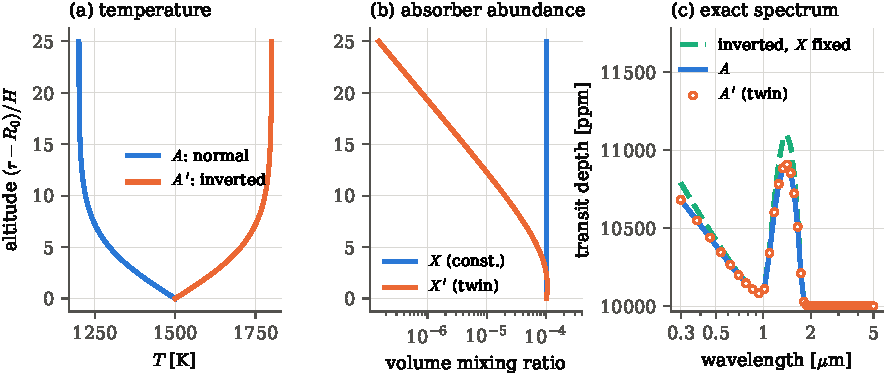
\includegraphics[width=\textwidth]{figures/inverted_twin.pdf}
\caption{The normal/inverted twin of \cref{thm:inverted} ($T_0=1200$\,K, $\Delta T=600$\,K,
$L=3H$). (a)~Temperature profiles. (b)~Constant mixing ratio of the normal atmosphere and
compensating profile \eqref{eq:comp} of the inverted one. (c)~Exact transit depths. The twin
(open circles) coincides with $\mathcal A$ to floating-point precision. Applying the inversion
without the compensation (dashed) changes the depth by up to $190$\,ppm.}
\label{fig:twin}
\end{figure}

\begin{figure}[t]
\centering
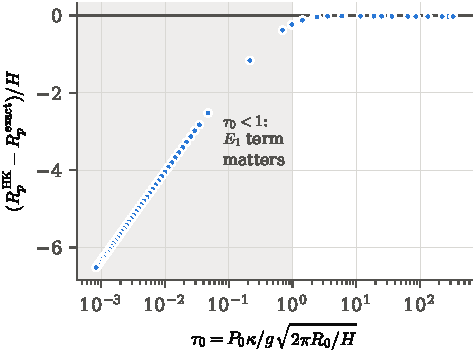
\includegraphics[width=0.55\textwidth]{figures/hk_vs_exact.pdf}
\caption{Analytic formula \eqref{eq:HK} minus the exact integral \eqref{eq:exact}, in units of
$H$, for the isothermal model, against $\tau_0$. For $\tau_0>10$ the two agree within $0.03H$.
For $\tau_0<1$ (shaded), the neglected $E_1(\tau_0)$ term and the opaque lower boundary
dominate.}
\label{fig:hk}
\end{figure}

\Cref{fig:twin} illustrates \cref{thm:inverted}. The compensating mixing ratio stays in
$[1.5\times10^{-7},1.04\times10^{-4}]$, within the bound $X'\le2X$ of
\cref{prop:admissible}. The maximum depth difference between the twins is $0$ to floating-point
precision. Without compensation, the inversion changes the depth by up to $190.5$\,ppm.
\Cref{cor:isotwin} with $c=1.5$ reproduces the depths to $2\times10^{-11}$\,ppm.
\Cref{fig:hk} shows that the analytic formula agrees with the exact integral to $0.027H$ at all
10 of the 60 wavelengths with $\tau_0>10$. Where $\tau_0<1$ it falls up to $6.5H$ below, which
is the regime of \cref{thm:E1}.

\section{Formalisation notes}\label{sec:lessons}

The development uses Lean~4 (v4.35.0) and Mathlib (v4.35.0). All headline theorems depend only
on the axioms \lean{propext}, \lean{Classical.choice} and \lean{Quot.sound}, as checked by
\lean{scripts/CheckAxioms.lean}, and no \lean{sorry} remains. \Cref{fig:lean} shows the Lean
statement of \cref{thm:profile}. Analytic ingredients come from Mathlib: the fundamental theorem
of calculus for hydrostatics, uniqueness of derivatives for \cref{lem:rigidity}, the mean value
theorem for \cref{thm:closure}, the intermediate value theorem for \cref{thm:singleband}, and
Bochner integration on $(1,\infty)$ for $E_1$.

\begin{figure}[t]
\small
\begin{alltt}
theorem temperature_profile_unidentifiable (hA : A.WellPosed) (T' : \(\mathbb{R}\to\mathbb{R}\))
    (hc : Continuous T') (hT' : \(\forall\) r, 0 < T' r) :
    \(\exists\) A' : Atmosphere \(\iota\), A'.WellPosed \(\wedge\) A'.T = T' \(\wedge\)
      A'.R0 = A.R0 \(\wedge\) A'.P0 = A.P0 \(\wedge\) A'.g = A.g \(\wedge\) A'.m = A.m \(\wedge\)
      (\(\forall\) i r, A'.speciesDensity i r = A.speciesDensity i r) \(\wedge\)
      \(\forall\) \(\sigma\) Rtop, A'.spectrum \(\sigma\) Rtop = A.spectrum \(\sigma\) Rtop
\end{alltt}
\caption{Lean statement of \cref{thm:profile} (\lean{ExoLean/ProfileDegeneracy.lean}).}
\label{fig:lean}
\end{figure}

\paragraph{Specification errors found by attempting proofs.}
Two of our own initial problem statements were wrong, and the proof attempts exposed both:
\begin{enumerate}
\item \emph{Power rigidity} was first stated without $r,C>0$. With $r=0$, any constant cloud
  satisfies $\kappa'=C\kappa^0$, so no family with a non-constant cone element could be rigid
  (\lean{not\_powerRigidUnrestricted}). The reduction theorem was true but vacuous. Since the
  physics only produces $r=H/H'>0$ and $C>0$, the corrected definition loses nothing.
\item \emph{Density identifiability} was first stated over all atmospheres. That class admits
  zero-thickness columns and pointwise modifications, which made the target false for trivial
  reasons (\lean{not\_densityProfilesIdentifiable}).
\end{enumerate}
In both cases the error did not show up in prose, and was found when a proof was attempted.
Identifiability conjectures are statements about \emph{all} parameter sets, so a single
overlooked edge case can make them vacuous or trivially false. We see this as an argument for
stating such conjectures formally.

\section{Open problems}\label{sec:open}

\begin{enumerate}
\item \textbf{Multi-band power rigidity} (\lean{GaussianBandsPowerRigid}, $|\iota|\ge2$).
  A plausible route is in three steps. First, extend $g=C f^r$ from the band to $\R$ by real
  analyticity, since $f>0$ everywhere. Second, compare asymptotics as $\lambda\to\infty$, where
  a unique slowest-decaying active band exists. Third, observe that this forces a band with the
  same centre but width $s/\sqrt r$ (cloud-free case) or $s/\sqrt2$ (cloudy case), which
  contradicts injectivity of the centres unless $r=1$.
\item \textbf{Single-species density identifiability}
  (\lean{DensityProfilesIdentifiableCts},
  non-proportional cross-sections). This needs Abel inversion together with uniqueness for
  Laplace-type transforms, and probably a monotonicity hypothesis.
\item \textbf{Relaxing the structural assumptions} of \cref{tab:lattice}: temperature-dependent
  cross-sections, an active background (which by \cref{thm:closure} removes the profile
  degeneracy at the level of densities), refraction, and variable gravity.
\end{enumerate}
Each target is stated as a Lean proposition, so a proof or a counterexample from a human or an
automated prover is checked mechanically.

\section{Conclusions}

Formalising transmission-spectrum forward models makes exact degeneracies into theorems with
explicit witnesses, and makes identifiability claims precise. In the exact model, the
temperature profile is entirely unconstrained when the cross-sections are temperature
independent and the background is invisible. That freedom vanishes once the composition is
closed. In the analytic model, three of seven parameters are identifiable. The remaining four
directions are an explicit gauge group, and its $(R_0,P_0)$ part is broken, by an exponentially
small amount, once the optically thick approximation is dropped. Between the two models, power
rigidity of the opacity cone is the right notion for multi-absorber identifiability.

\section*{Acknowledgements}
The Lean development, numerical scripts and this manuscript were produced with the assistance
of Claude (Anthropic), an AI system. Every theorem stated here is checked by the Lean kernel.

\section*{Appendix: map from results to Lean}
\begin{table}[H]
\centering\footnotesize
\begin{tabularx}{\textwidth}{@{}lXl@{}}
\toprule
Result & Lean name & File\\\midrule
\Cref{lem:bridge} & \lean{Atmosphere.speciesDensity\_of\_isothermal\_isochemical} & \lean{Assumptions}\\
\Cref{thm:factor} & \lean{Atmosphere.spectrum\_eq\_of\_speciesDensity\_eq} & \lean{Atmosphere}\\
\Cref{thm:profile} & \lean{Atmosphere.temperature\_profile\_unidentifiable} & \lean{ProfileDegeneracy}\\
\Cref{prop:admissible} & \lean{Atmosphere.PhysicalVMR.retemper} & \lean{ProfileDegeneracy}\\
\Cref{cor:isotwin}, \cref{thm:inverted} & \lean{Atmosphere.isothermal\_twin}, \lean{Atmosphere.exists\_inverted\_twin} & \lean{ProfileExamples}\\
\Cref{thm:closure} & \lean{Atmosphere.T\_eq\_of\_speciesDensity\_eq} & \lean{ProfileClosure}\\
\Cref{prop:gauge} & \lean{Iso.transitRadius\_referenceGauge}, \lean{Iso.transitRadius\_normalization}, \lean{Iso.transitRadius\_T\_g}, \lean{Iso.transitRadius\_T\_m} & \lean{Analytic}\\
\Cref{lem:rigidity}, \cref{thm:fibre} & \lean{logAffine\_rigidity}, \lean{Iso.transitRadius\_fibre} & \lean{Identifiability}\\
\Cref{sec:regimes} & \lean{Iso.grey\_temperature\_unidentifiable}, \lean{Iso.lecavelier\_slope}, \lean{Iso.powerLaw\_slope\_degeneracy} & \lean{Degeneracies}\\
\Cref{thm:reduction,thm:powertwin} & \lean{Iso.scaleHeight\_eq\_of\_powerRigid}, \lean{Iso.exists\_powerRelated\_twin} & \lean{Rigidity}\\
\Cref{thm:singleband} & \lean{powerRigid\_of\_unique} & \lean{GaussianRigidity}\\
\Cref{thm:E1} & \lean{Iso.transitRadiusE1\_referenceGauge}, \lean{expIntegralE1\_strictAntiOn} & \lean{E1Gauge}\\
\Cref{sec:density} & \lean{not\_densityProfilesIdentifiableCts\_of\_proportional} & \lean{DensityTargets}\\\bottomrule
\end{tabularx}
\caption{Results and their Lean counterparts (all in namespace \lean{ExoLean}).}\label{tab:map}
\end{table}

\bibliographystyle{plainnat}
\bibliography{references}

\end{document}
